\documentclass[a4]{ltjsarticle}
\usepackage{amsmath, amssymb, amsfonts}
\usepackage{graphicx}
\usepackage[linktocpage,
						colorlinks=true,
						linkcolor=blue,
						citecolor=blue,
						urlcolor=blue]{hyperref}

% 式番号に節を追加
\makeatletter
	\renewcommand{\theequation}{\arabic{section}.\arabic{equation}}
	\@addtoreset{equation}{section}
\makeatother

\newcommand{\deriv}{\frac{d}{dt}}
\newcommand{\pathint}[1]{\int \mathcal{D}#1 \ }
\newcommand{\average}[1]{\langle #1 \rangle}
\newcommand{\combination}[2]{{}_{#1} \mathrm{C}_{#2}}
\newcommand{\sgn}{\mathrm{sgn}}

\begin{document}
	\title{量子カオス理論におけるSachdev--Ye--Kitaev模型}
\author{西村 滉祐}
\date{}
\maketitle

\begin{abstract}
	これは修論です。
\end{abstract}

\thispagestyle{empty}
\pagebreak

	\setcounter{page}{1}
	\tableofcontents
	\pagebreak
	\section{はじめに}
ここに序論を書く。
\begin{align}
test function
\label{eq:test}
\end{align}
\eqref{eq:test}はテストです。

\pagebreak
	\section{2点関数}
\subsection{シュウィンガー・ダイソン方程式}
\begin{figure}[ht]
  \centering
  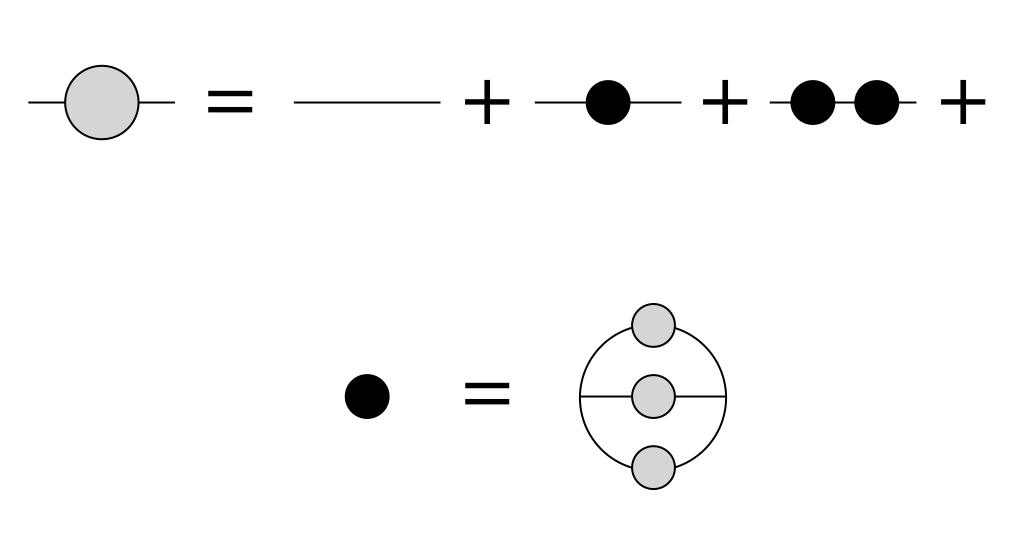
\includegraphics[width=14cm]{figures/melonDiagram}
  \caption{ラージN極限において2点関数に寄与する最初の補正ダイアグラム.
  特に$q=4$の場合について描画している. 灰色の丸と黒い丸はそれぞれ完全な2点関数および
  1粒子相互作用を表している.}
  \label{fig:melonDiagram}
\end{figure}

SYK模型の作用は
\begin{align}
  I = \int dt\ \left(\frac{1}{2}\sum_{i = 1}^{N} \psi_i \deriv \psi_i
		- \frac{1}{4!} \sum_{i,j,k,l = 1}^{N} J_{ijkl} \psi_i\psi_j\psi_k\psi_l
    \right)
\end{align}
である。
これを$J_{ijkl}$について期待値を取り、その後フェルミオンを積分するために
2つのbi-local場$G(t_1, t_2)$, $\Sigma(t_1, t_2)$を導入すると
\begin{align}
  \frac{I_{\mathrm eff}}{N} =
		- \frac{1}{2}\log\det\left(\deriv - \Sigma\right)
		+ \frac{1}{2}\int dt_1dt_2\ \left(\Sigma G - \frac{J^2}{4}G^4\right)
  \label{eq:effectiveAction}
\end{align}
を得る\footnote{詳しい計算は\ref{app:effective_action}を参照すること.}。
\eqref{eq:effectiveAction}式の停留点が次式のシュウィンガー・ダイソン方程式を与える:
\begin{align}
  G(\omega)^{-1} = -i\omega - \Sigma(\omega),
  \hspace{30pt}
  \Sigma(t) = J^2G(t)^3
  \label{eq:SDeq}
\end{align}

なお、SYK模型では4つのフェルミオンが相互作用するとしているが、その数を$q$として一般化しても
有効作用やシュウィンガー・ダイソン方程式は計算する事ができ、それぞれ
\begin{align}
  \frac{I_{\mathrm eff}}{N} =
		- \frac{1}{2}\log\det\left(\deriv - \Sigma\right)
		+ \frac{1}{2}\int dt_1dt_2\ \left(\Sigma G - \frac{J^2}{q}G^q\right)
  \label{eq:effectiveActionWithGeneral_q}
\end{align}
\begin{align}
  G(\omega)^{-1} = -i\omega - \Sigma(\omega),
  \hspace{30pt}
  \Sigma(t) = J^2G(t)^{q-1}
  \label{eq:SDeqWithGeneral_q}
\end{align}
である。さらに複数の$q$について相互作用項を足し合わせたような一般化したSYK模型も
調べられており、\cite{gross}にて詳しく論じられている。

ラージ$N$極限を施したSYK模型において、リーディングオーダーで2点関数に寄与する
ファインマンダイアグラムは「メロンダイアグラム」と呼ばれている
\footnote{このメロンはwatermelonのmelonであってメロンではないらしい.
どの辺がスイカなのかはよく分からない.}。
\eqref{eq:SDeq}式は解析的には解けないが、数値的には可能であり、
図\ref{fig:melonDiagram}のダイアグラムのように再帰的に計算を走らせる事で
2点関数のグラフをプロットできる。

\subsection{共形不変性}

\subsection{ラージ$q$リミット}

\subsubsection{リーディングオーダー}

\subsubsection{サブリーディングオーダー}





\pagebreak

	\section{4点関数\label{sec:fourpointfunc}}
ここでは強結合領域$\beta J \gg 1$における4点関数の解析解について述べる。
特にラージ$N$におけるリーディングオーダー$\mathcal{F}$を調べるのだが、ダイアグラムは書き下せても
一般的な解析解は知られていない。
$\mathcal{F}$に寄与するダイアグラムはラダーダイアグラムと呼ばれるものであり、$\mathcal{F}$は
その総和で与えられる。
$n$個、および$n+1$個の輪を持つダイアグラムの間には積分核$K$で与えられる漸化式が存在し、
ダイアグラムの総和は$K$の幾何級数で与えられる。
従ってリーディングオーダーは$\mathcal{F} = \frac{1}{1-K}\mathcal{F}_0$で与えられる。
ここで$\mathcal{F}_0$は輪を持たないダイアグラムである。
概念的には簡単であるが、$K$の作用する関数空間についてある程度理解する必要があり、
実際の計算はとても複雑である。
そこで2点関数では共形極限における解析解$G_c$が調べられている事を思い出し、
4点関数でもそれを用いる事にする。
基本的に4点関数のリーディングオーダー$\mathcal{F}$は2点関数で構成されるので、
原理的には$G_c$を用いて解析は可能であり、実際に解を導く。
ただしそれでも、そこまでの道のりがかなり長い。
一次元における共形対称性は$SL(2, \mathbb{R})$であり、これを$K$の対角化において活用する。
これによって一応の計算結果が示されるが、結果の表式に存在する級数は
低エネルギー極限で計算した事に起因する技術上の発散項を含む。
この発散項は、$K = 1$となるような$K$の固有関数の存在によってもたらされる。
この発散を処理するためには、リパラメトリゼーション不変性の成り立つ低エネルギー極限から
少し高エネルギー側にずれる必要がある。
すなわち、有限な解ではリパラメトリゼーション不変性は自発的にも、また陽にも破れる。
発散項はこれによって有限になり、共形対称性を持たない。
disorder averageを取る事によって最も一般的な4点関数は
\begin{align}
	\average{\psi_i(t_1)\psi_i(t_2)\psi_j(t_3)\psi_j(t_4)}
\end{align}
という形に制限される。
これを$i$と$j$について平均を取ったものを考える:
\begin{align}
	\frac{1}{N^2}\sum_{i,j=1}^{N}\average{T\psi_i(t_1)\psi_i(t_2)\psi_j(t_3)\psi_j(t_4)}
	= G(t_{12})G(t_{34}) + \frac{1}{N}\mathcal{F}(t_1, \cdots, t_4).
	\label{eq:fourpointfunc}
\end{align}
以下では$\mathcal{F}$について解析する。

\begin{figure}[h]
	\centering
	\vspace{1cm}
	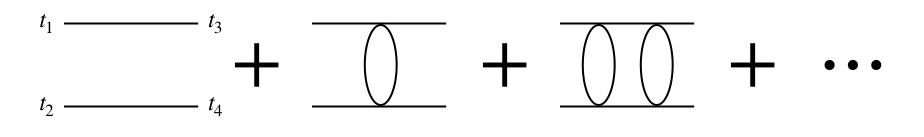
\includegraphics[width=13cm]{figures/ladderDiagram}
	\caption{\eqref{eq:fourpointfunc}式の$1/N$の項を表すダイアグラム。
		特に$q=4$の場合について描画した。ラダーダイアグラムと呼ぶ。}
	\label{fig:ladderdiagram}
\end{figure}

$\mathcal{F}$を表すダイアグラムはラダーダイアグラムである(図\ref{fig:ladderdiagram})。
$n$個の輪があるものを$\mathcal{F}_n$とすると、計算するべきは
\begin{align}
	\mathcal{F} = \sum_n \mathcal{F}_n
\end{align}
である。
図\ref{fig:ladderdiagram}の最初にある輪を持たないラダーダイアグラムは単なるプロパゲーターの積である:
\begin{align}
	\mathcal{F}_0(t_1, \cdots, t_4) = -G(t_{13})G(t_{24}) + G(t_{14})G(t_{23}).
\end{align}
次に並ぶ、輪を1個だけ持つラダーダイアグラムでは、輪の端の位置について積分した形で与えられる:
\begin{align}
	\mathcal{F}_1(t_1, &\cdots, t_4)\nonumber\\
	&= J^2(q - 1)\int dtdt'\ \left(
		G(t_1 - t)G(t_2 - t')G(t - t')^{q-2}G(t - t_3)G(t' - t_4) - (t_3 \leftrightarrow t_4)
	\right).
\end{align}
積分の前にある$q-1$という因子は、どの線をレールや輪にするかのパターン数に起因する。
上述した2つのラダーダイアグラム$\mathcal{F}_0$、$\mathcal{F}_1$に限らず、
全てのラダーダイアグラムは$1/N$に比例する。

あるラダーダイアグラム$\mathcal{F}_n$と次の$\mathcal{F}_{n+1}$の間には
\begin{align}
	\mathcal{F}_{n+1}(t_1, \cdots, t_4)
	= \int dtdt'\ K(t_1, t_2; t, t')\mathcal{F}_n(t, t', t_3, t_4)
	\label{eq:F_n+1_and_F_n}
\end{align}
という漸化式的な関係がある。
ここで積分核$K$は
\begin{align}
	K(t_1, t_2; t_3, t_4) = -J^2(q-1)G(t_{13})G(t_{24})G(t_{34})^{q-2}
	\label{eq:def_of_K}
\end{align}
である。
\eqref{eq:F_n+1_and_F_n}式の計算では、$K$の最初の2つの変数を1つ目の添字、残りの2つを2つ目の添字
と見なす事によって積分を行列計算としてしまうのが便利である(行列$K$は2変数反対称関数の空間に作用する)。
こうする事で全てのラダーダイアグラムの総和を
\begin{align}
	\mathcal{F}
	= \sum_{n=0}^{\infty}\mathcal{F}_n
	= \sum_{n=0}^{\infty}K^n \mathcal{F}_0
	= \frac{1}{1 - K}\mathcal{F}_0
	\label{eq:geometric_series_of_F}
\end{align}
という様に表す事ができる。
これを更に計算するために、以下では$K$を対角化する事を考える。
\eqref{eq:def_of_K}式による定義では$K$は対称行列ではないが、
次のような操作により対称化する事が可能である:
\begin{align}
	\tilde{K}(t_1, t_2; t_3, t_4) \equiv
	|G(t_{12})|^{\frac{q-2}{2}}K(t_1, t_2; t_3, t_4)|G(t_{34})|^{\frac{2-q}{2}}.
	\label{eq:symmetric_K}
\end{align}
従って$K$は固有関数(固有ベクトル)の完全系を持つとして良い。

\subsection{$K_c$の対角化}
ここまでの話は一般の$\beta J$について成り立つ。
解析を進めるために、以下では共形対称性の成り立つ極限$\beta J \gg 1$で考える。
よって2点関数は$\eqref{eq:conformal_ansatz}$式の$G_c(t)$で与えられる。
\eqref{eq:conformal_ansatz}式を\eqref{eq:def_of_K}式に代入すると、
$K$の共形不変なものとして
\begin{align}
	K_c(t_1, t_2; t_3, t_4)
	= -\frac{1}{\alpha_0}
		\frac{\sgn(t_{13})\sgn(t_{24})}{|t_{13}|^{2\Delta}|t_{24}|^{2\Delta}|t_{34}|^{2-4\Delta}}
	\label{eq:confomarl_K}
\end{align}
を得る。ここで
\begin{align}
	\alpha_0 \equiv \frac{2\pi q}{(q-1)(q-2)\tan\frac{\pi}{q}}
	\label{eq:alpha_0}
\end{align}
である。
$K_c$を対角化した暁には、実は固有関数の中に固有値$k_c(h) = 1$を持つものも存在する。
従って\eqref{eq:geometric_series_of_F}式の級数は発散するが、これは共形極限から摂動的に少し
ずれる事によって対処する事ができる。
それを議論するまでは、ひとまず\eqref{eq:confomarl_K}式を用いる事にする。

$K_c$の対角化では共形不変性を活用する事になる。
SYK模型は時間1次元しか持たないので、1次元共形場理論$\mathrm{CFT}_1$であり
\footnote{1次元の場の量子論は本質的に量子力学なので、
Conformal Quantum Mechanicsの頭文字を取ってCQMと表記する事もある。}、
共形変換群は$SL(2, \mathbb{R})$で与えられる\cite{andrzejewski}:
\begin{align}
	\hat{D} = -t\partial_t - \Delta,\hspace{20pt}
	\hat{P} = \partial_t,\hspace{20pt}
	\hat{K} = t^2\partial_t + 2t\Delta,
\end{align}
\begin{align}
	[\hat{D}, \hat{P}] = \hat{P},\hspace{20pt}
	[\hat{D}, \hat{K}] = -\hat{K},\hspace{20pt}
	[\hat{P}, \hat{K}] = -2\hat{D}.
\end{align}
これらの生成子は$K_c$と交換し、
\begin{align}
	(\hat{D}_1 + \hat{D}_2)K_c(t_1, t_2; t_3, t_4)
	= K_c(t_1, t_2; t_3, t_4)(\hat{D}_3 + \hat{D}_4)
	\label{eq:D_and_Kc}
\end{align}
となる。
ただし、この可換性を示す計算の際に現れる表面項の取扱いには注意を要する。
$K_c$の固有関数を$\Psi_h$とすると、固有値方程式は
\begin{align}
	\int dt_1dt_2\ \Psi_h(t_1, t_2) K(t_1, t_2; t_3, t_4)
	= k_c(h)\Psi_h(t_3, t_4)
	\label{eq:eigen_eq_of_Kc}
\end{align}
となり、\eqref{eq:D_and_Kc}式は正確に書けば
\begin{align}
	\int dt_1 dt_2\ \left[(\hat{D}_1 + \hat{D}_2)\Psi_h(t_1, t_2)\right]
	&K_c(t_1, t_2; t_3, t_4)\nonumber\\
	&= (\hat{D}_3 + \hat{D}_4)\int dt_1dt_2\ \Psi_h(t_1, t_2) K_c(t_1, t_2; t_3, t_4)
	\nonumber\\
	&= k_c(h)\left[(\hat{D}_3 + \hat{D}_4)\Psi_h(t_3, t_4)\right]
\end{align}
である。この最初の行の積分を実行する際に現れる表面項は、
後に$K_c$の固有関数は超幾何関数${}_2F_1$のある特定の線型結合である事が判明するが、
これを用いた場合のみ消滅する。
$\hat{P}$や$\hat{K}$についても同様である。

この対称性により、まずラダーダイアグラム$\mathcal{F}_n$は$SL(2, \mathbb{R})$不変の
複比(cross ratio)
\begin{align}
	\chi = \frac{t_{12}t_{34}}{t_{13}t_{24}}
\end{align}
の関数である事が示唆される。
これは$\mathcal{F}_0$が共形4点関数のように変換するからである。
この性質は$SL(2, \mathbb{R})$不変の演算子を作用させても変わらない。
従って$K_c(t_1, t_2; t_3, t_4)$とする代わりに$K_c(\chi; \tilde{\chi})$とする事ができる。
2つ目の示唆は、$K_c$が次式で与えられるカシミール演算子$C_{1+2}$と可換というものである:
\begin{align}
	C_{1+2}
	&= (\hat{D}_1 + \hat{D}_2)^2
	- \frac{1}{2}(\hat{K}_1 + \hat{K}_2)(\hat{P}_1 + \hat{P}_2)
	- \frac{1}{2}(\hat{P}_1 + \hat{P}_2)(\hat{K}_1 + \hat{K}_2)\nonumber\\
	&= 2(\Delta^2 - \Delta) - \hat{K}_1\hat{P}_2 - \hat{P}_1\hat{K}_2 + 2\hat{D}_1\hat{D}_2.
	\label{eq:casimir_operator}
\end{align}
スペクトラムに縮退はないため、これは$K_c$の固有関数が$C_{1+2}$のそれと同じである事を意味する。
\eqref{eq:geometric_series_of_F}式を$C_{1+2}$の固有関数$\Psi_h(\chi)$で展開すれば、
何らかの内積を用いて
\begin{align}
	\mathcal{F}(\chi)
	= \sum_h \Psi_h(\chi)\frac{1}{1 - k_c(h)}
		\frac{\innerprod{\Psi_h}{\mathcal{F}_0}}{\innerprod{\Psi_h}{\Psi_h}}
	\label{eq:final_F_chi}
\end{align}
と変形できる。
よって我々が行うべき仕事は$\Psi_h$と$k_c(h)$を求め、そして内積を計算する事である。
そのために、まず$\chi$の関数としての$\mathcal{F}_n$の性質を調べる事から始める。

\subsubsection{$\mathcal{F}_n(\chi)$の性質}
共形極限では、ラダーダイアグラム$\mathcal{F}_n$は$SL(2, \mathbb{R})$変換のもとで
次元$\Delta$を持つ4点関数として振る舞う:
\begin{align}
	\mathcal{F}_n(t_1, t_2; t_3, t_4)
	= G_c(t_{12})G_c(t_{34})\mathcal{F}_n(\chi).
\end{align}
$t_1$と$t_2$の間、および$t_3$と$t_4$の間の反対称性、さらに$(t_1, t_2)$と$(t_3, t_4)$の間の対称性
や$SL(2, \mathbb{R})$変換を駆使すると、$t_1 = 0$、$t_3 = 1$、$t_4 = \infty$さらに$t_2 > 0$
という様に移す事ができ、$\chi = t_2$の値を正であるとして制限できる。
\eqref{eq:fourpointfunc}式の時間順序積の存在により、$\chi > 1$か$\chi < 1$かによって
\begin{align}
	\mathcal{F}_n(\chi)
	\approx \left\{
		\begin{array}{l}
			+\average{\psi_j(\infty)\psi_j(1)\psi_i(\chi)\psi_i(0)}\hspace{20pt}
			0 < \chi < 1\\
			-\average{\psi_j(\infty)\psi_i(\chi)\psi_j(1)\psi_i(0)}\hspace{20pt}
			1 < \chi < \infty
		\end{array}
	\right.
\end{align}
となる。

$\chi > 1$の領域では、ある離散的な対称性が存在する。
これを見るには
\begin{align}
	\frac{t-2}{t} = \tan \frac{\theta}{2}
\end{align}
として$t$を円周上に写像すると良い。
$t = 0, 1, \infty$はそれぞれ$\theta = -\pi, -\frac{\pi}{2}, \frac{\pi}{2}$に写される。
$t_2 = \chi$はある$\theta$が対応する(図\ref{fig:circle})。
対称性$\theta \to -\theta$によって$\chi \to \frac{\chi}{\chi - 1}$となる。
\begin{figure}[ht]
	\centering
	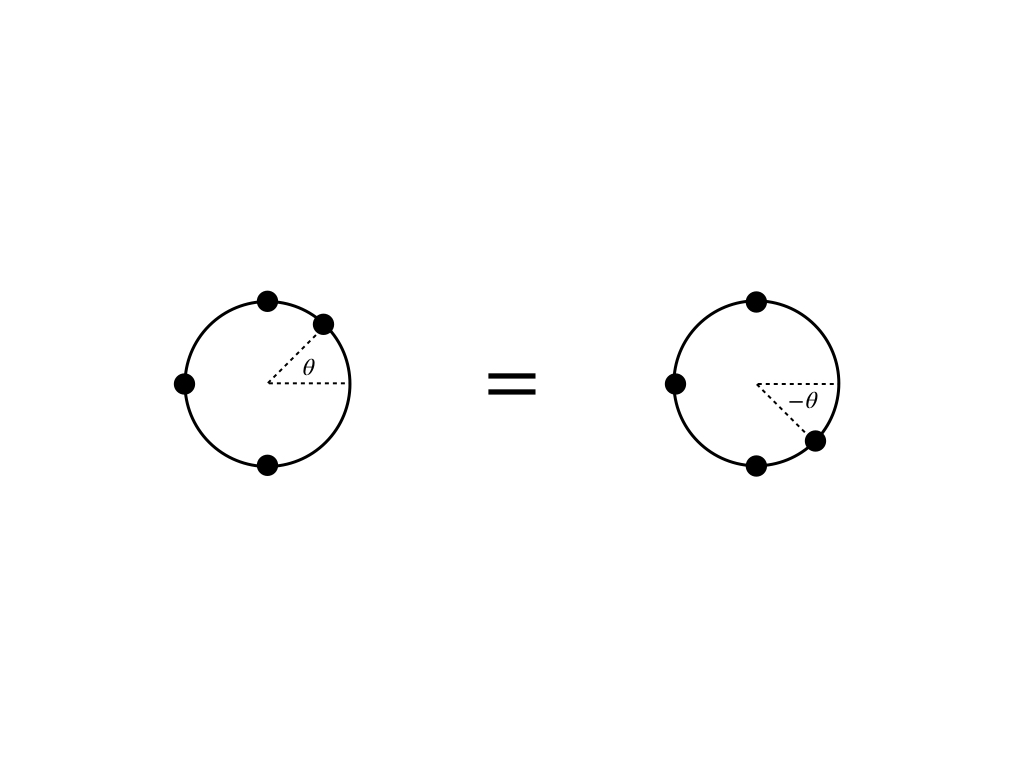
\includegraphics[width=11cm]{figures/circle}
	\caption{$\theta \to -\theta$という対称性は
		$\chi > 1$において$\chi \to \frac{\chi}{\chi - 1}$と対応する。}
	\label{fig:circle}
\end{figure}

これは$\chi > 1$では$\mathcal{F}(\chi) = \mathcal{F}(\frac{\chi}{\chi - 1})$が成り立つ
事を意味する。
この変換は$1 < \chi < 2$の区間を$2 < \chi < \infty$へと写す事に注意すると、
$\mathcal{F}(\chi)$を決定するには$0 < \chi < 2$という区間で十分である事に気付く。
また$\chi = 2$は固定点なので、$\mathcal{F}$の一階微分の$\chi = 2$における値は0であるという条件もつく。

$\mathcal{F}_{n+1}$と$\mathcal{F}_n$の間の関係式
\eqref{eq:F_n+1_and_F_n}式を$\chi$を用いて書き直すと
\begin{align}
	\mathcal{F}_{n+1}(\chi)
	= \int_0^2 \frac{d\tilde{\chi}}{\tilde{\chi}^2}\ 
		K_c(\chi; \tilde{\chi})\mathcal{F}_n(\chi)
	\label{eq:F_n+1_and_F_n_in_chi}
\end{align}
となる。
$K_c(\chi; \tilde{\chi})$は次式で与えられる:
\begin{align}
	K_c(\chi; \tilde{\chi}) = \frac{1}{\alpha_0}\left[
		\frac{\chi^{2\Delta}\tilde{\chi}^{2\Delta}}{|\chi - \tilde{\chi}|^{2\Delta}}
		m(\chi, \tilde{\chi}) + \sgn(\tilde{\chi} - 1)
		\frac{\chi^{2\Delta}\tilde{\chi}^{2\Delta}}
			 {|\chi + \tilde{\chi} - \chi\tilde{\chi}|^{2\Delta}}
		m\left(\chi, \frac{\tilde{\chi}}{\tilde{\chi} - 1}\right)
	\right].
\end{align}
ここで$m(\chi, \tilde{\chi})$は次のような超幾何関数${}_2F_1$で与えられる
$\chi$と$\tilde{\chi}$に関して対称な関数である:
\begin{align}
	z \equiv \frac{1 - \min(\chi, \tilde{\chi})}{|\chi - \tilde{\chi}|},\hspace{20pt}
	B_h(x) = \frac{\Gamma(h)^2}{\Gamma(2h)}x^h\ {}_2F_1(h, h, 2h, x)
\end{align}
という2つの記号を導入して、
\begin{align}
	m(\chi, \tilde{\chi})
	= \frac{2\pi}{\sin 2\pi\Delta}{}_2F_1(1 - 2\Delta, 2\Delta, 1, z)
	- B_{2\Delta}\left(\frac{1}{1 - z}\right)
	- B_{1 - 2\Delta}\left(\frac{1}{1 - z}\right)
	\hspace{20pt} z \leq 0,
\end{align}
\begin{align}
	m(\chi, \tilde{\chi})
	= -\frac{2\pi}{z^{2\Delta}\sin 2\pi\Delta}{}_2F_1\left(
		2\Delta, 2\Delta, 1, \frac{z - 1}{z}\right)
	+ \frac{2\pi}{\sin 2\pi\Delta}{}_2F_1(2\Delta, 1 - 2\Delta, 1, z)
	\hspace{20pt} 0 \leq z \leq 1,
\end{align}
\begin{align}
	m(\chi, \tilde{\chi})
	= -\frac{2\pi}{\sin 2\pi\Delta}{}_2F_1(2\Delta, 1 - 2\Delta, 1, 1 - z)
	- B_{2\Delta}\left(\frac{1}{z}\right)
	- B_{1 - 2\Delta}\left(\frac{1}{z}\right)
	\hspace{20pt} 1 \leq z 
\end{align}
である。

\subsubsection{カシミール演算子$C_{1+2}の固有関数$}

次にカシミール演算子$C_{1+2}$の固有関数を求める。
\eqref{eq:casimir_operator}式から、$C_{1+2}$は
\begin{align}
	C_{1+2}\frac{1}{|t_{12}|^{2\Delta}}f(\chi)
	= \frac{1}{|t_{12}|^{2\Delta}}\mathcal{C}f(\chi),\hspace{20pt}
	\mathcal{C} = \chi^2(1 - \chi)\partial_{\chi}^2 - \chi^2\partial_{\chi}
\end{align}
を満たす。
$\mathcal{C}$の固有値を$h(h-1)$とすると、固有値方程式は$\mathcal{C}f = h(h-1)f$である。
この一般解は超幾何関数${}_2F_1$を用いて
\begin{align}
	\chi^h{}_2F_1(h, h, 2h, \chi),\hspace{30pt}
	x^{1-h}{}_2F_1(1-h, 1-h, 2-2h, \chi)
	\label{eq:eigenfunctions_of_C}
\end{align}
という2つの解の線型結合となる。
それで張られる空間は$f'(2) = 0$となるような関数の空間である。
またこの関数空間の内積は\eqref{eq:F_n+1_and_F_n_in_chi}式より
\begin{align}
	\innerprod{g}{f} = \int_0^2 \frac{d\chi}{\chi^2}g^*(\chi)f(\chi)
	\label{eq:innerproduct}
\end{align}
のように与えられる。規格化はこの内積から計算される。
$\mathcal{C}$がエルミート演算子であるための条件は
\begin{align}
	0
	= \innerprod{g}{\mathcal{C}f} - \innerprod{\mathcal{C}g}{f}
	= \int_0^2 d\chi\ \frac{d}{d\chi}\left[
		g^*(\chi)(1 - \chi)\frac{d}{d\chi}f(\chi)
		- \frac{d}{d\chi}g^*(\chi)(1 - \chi)f(\chi)
	\right]
\end{align}
である。
$\chi = 2$では$f$や$g^*$の一階微分が0になる事から表面項は消える。
また$\chi = 0$においても$f$や$g^*$は$\chi^{1/2}$よりも速く0となるという条件を課す事で消滅する。
加えて\eqref{eq:eigenfunctions_of_C}式の固有関数は$\chi = 1$にて対数発散が存在するため、
もう1つの条件を課す必要がある。
即ち、特異点を打ち消すためには
\begin{align}
	f &\approx A + B\log(1 - \chi)\hspace{20pt}\mathrm{for\ \ }\chi \to 1^-,\nonumber\\
	f &\approx A + B\log(\chi - 1)\hspace{20pt}\mathrm{for\ \ }\chi \to 1^+\nonumber
\end{align}
のように定数項と対数の項が1に近づくにつれ相殺していなければならない。

以上を踏まえて、カシミール演算子$C_{1+2}$の固有関数$\Psi_h(\chi)$は次のように書き下す事ができる。
まず$1 < \chi$の時は
\begin{align}
	\Psi_h(\chi)
	= \frac{\Gamma\left(\frac{1}{2} - \frac{h}{2}\right)\Gamma\left(\frac{h}{2}\right)}
		{\sqrt{\pi}}
	{}_2F_1\left(\frac{h}{2},\frac{1}{2} - \frac{h}{2},\frac{1}{2},
	\frac{(2 - \chi)^2}{\chi^2}\right)
	\label{eq:Psi_h_for_chi>1}
\end{align}
である。
また$\chi < 1$の時は
\begin{align}
	\Psi_h(\chi)
	= A\frac{\Gamma(h)^2}{\Gamma(2h)}\chi^h\ {}_2F_1(h, h, 2h, \chi)
	+ B\frac{\Gamma(1-h)^2}{\Gamma(2 - 2h)}\chi^{1-h}\ {}_2F_1(1-h, 1-h, 2-2h, \chi)
	\label{eq:Psi_h_for_chi<1}
\end{align}
である。ここで$A$と$B$は
\begin{align}
	A = \frac{1}{\tan\frac{\pi h}{2}}\frac{\tan\pi h}{2},\hspace{20pt}
	B = A(1 - h) = -\tan\frac{\pi h}{2}\frac{\tan\pi h}{2}
\end{align}
で与えられる。
$\chi > 1$と$\chi < 1$の両方の場合において$\Psi_h = \Psi_{1-h}$という性質を持つ。
最後に$\chi \to 0$で$\Psi_h$は$\chi^{1/2}$と同じかそれ以上に速く0に近づくという条件から、
$h$について次の2つの解が存在する:
1つ目は$h = \frac{1}{2} + is$というものである。
この時$\Psi_h(\chi)$は$1 < \chi$で単調関数であり、また$1 > \chi$で振動する(非常に多く振動する)。
2つ目は$h = 2n\ (n \in \mathbb{N})$であり、定数$B$は消滅する。この解もまた
$0 < 1 < \chi$で単調関数であり、$1 > \chi$で振動する(0を$n$回横切る)。

\subsubsection{$K_c$の固有値}
$C_{1+2}$の固有関数$\Psi_h$に縮退はないため、$K_c$と$C_{1+2}$が可換である事から$\Psi_h$は
$K_c$の固有関数でもある。
原理的には\eqref{eq:eigen_eq_of_Kc}式から固有値$k_c(h)$を計算できるが、
ここではもっと単純な方法を取る。
固有値$h(h-1)$を持つ$C_{1+2}$の固有関数は2つのフェルミオンの共形3点関数の形を持つ:
\begin{align}
	\frac{\sgn(t_{12})}{|t_{10}|^h|t_{20}|^h|t_{12}|^{2\Delta - h}}.
\end{align}
これは任意の$t_0$や$h$において$K_c$の固有関数である。
$SL(2, \mathbb{R})$を用いて$t_0$を動かす事が可能なため、固有値$k_c(h)$は$h$にのみ依存する。
特に$t_0$を無限大に持っていけば、固有値は\eqref{eq:confomarl_K}式より
\begin{align}
	k_c(h)
	= \int dt_1 dt_2\ K_c(1, 0; t_1, t_2)\frac{\sgn(t_{12})}{|t_{12}|^{2\Delta - h}}
	= -\frac{1}{\alpha_0}\int dt_1dt_2\ 
	\frac{\sgn(1 - t_1)\sgn(-t_2)\sgn(t_{12})}
	{|1-t_1|^{2\Delta}|t_2|^{2\Delta}|t_{12}|^{2-2\Delta-h}}
\end{align}
となる。
この積分の実行には
\begin{align}
	\frac{\sgn(t)}{|t|^a} = \int\frac{\d\omega}{2\pi}
		e^{-i\omega t}c(a)|\omega|^{a-1}\sgn(\omega),\hspace{20pt}
		c(a) = 2i2^{-a}\sqrt{\pi}
		\frac{\Gamma\left(1-\frac{a}{2}\right)}{\Gamma\left(\frac{1}{2}+\frac{a}{2}\right)}
\end{align}
を用いると良い。
結果は
\begin{align}
	k_c(h) = \frac{1}{\alpha_0}\frac{c(2-2\Delta-h)}{c(2\Delta-h)}c(2\Delta)^2
	\label{eq:eigenvalue_of_Kc}
\end{align}
となる。
$k_c(h)$は全ての$h = \frac{1}{2} + is$や$h = 2n$で実数となる。
特に連続的なスペクトラムに対しては負、離散的なスペクトラムだと正となる。
$q = 4, \infty, 2$の場合について具体的な式は
\begin{align}
	k_c(h) &= -\frac{3}{2}\frac{\tan\frac{\pi(h - 1/2)}{2}}{h - \frac{1}{2}}
	\hspace{30pt}q = 4,\\
	k_c(h) &= \frac{2}{h(h-1)}
	\hspace{61pt}q = \infty,\\
	k_c(h) &= -1
	\hspace{87pt}q = 2
\end{align}
となる。特に$q = 4, \infty$の時$k_c(h=2) = 1$となり、\eqref{eq:geometric_series_of_F}
の級数が発散する。
この$h = 2$についての正しい取り扱いは後に議論する。

\subsubsection{$\innerprod{\Psi_h}{\Psi_h}$と$\innerprod{\Psi_h}{\mathcal{F}_0}$}

次に\eqref{eq:final_F_chi}式の計算に必要な2つの内積
$\innerprod{\Psi_h}{\Psi_h}$と$\innerprod{\Psi_h}{\mathcal{F}_0}$を求める。
連続的なスペクトラム$h = \frac{1}{2} + is$に関しては
\begin{align}
	\innerprod{\Psi_h}{\Psi_h} = \frac{\pi\tan\pi h}{4h-2}2\pi\delta(s - s')
\end{align}
で与えられ、また離散的なスペクトラム$h = 2n, n\in\mathbb{N}$に関しては
\begin{align}
	\innerprod{\Psi_h}{\Psi_h} = \frac{\delta_{hh'}\pi^2}{4h-2}
\end{align}
となる。

$\chi$の関数としての$\mathcal{F}_0$は
\begin{align}
	\mathcal{F}_0(\chi) = \left\{
	\begin{array}{l}
		-\chi^{2\Delta} + \left(\frac{\chi}{1 - \chi}\right)^{2\Delta}
		\hspace{20pt}0 < \chi < 1,\\
		-\chi^{2\Delta} - \left(\frac{\chi}{\chi - 1}\right)^{2\Delta}
		\hspace{20pt}1 < \chi < \infty
	\end{array}\right.
\end{align}
で与えられる。
以下では内積$\innerprod{\Psi_h}{\mathcal{F}_0}$の計算には連続的なスペクトラムについてのみ考える。
離散的なスペクトラムの場合は$h$について解析接続する事で得られる。
固有関数$\Psi_h$は連続スペクトラムにおいて次のような積分表示を持つ:
\begin{align}
	\Psi_h(\chi) = \frac{1}{2}\int_{-\infty}^{\infty}dy\ 
	\frac{|\chi|^h}{|y|^h|\chi - y|^h|1 - y|^{1-h}}.
\end{align}
この積分表示を用いて$\innerprod{\Psi_h}{\mathcal{F}_0}$の積分を行う。
$\chi\to\frac{\chi}{\chi-1}$の変換で$\Psi_h(\chi) = \Psi_h\left(\frac{\chi}{\chi-1}\right)$
であるが、$\mathcal{F}_0$はこの変換で、$\chi > 1$の時は対称、$\chi < 1$の時は反対称となる。
この性質を用いると
\begin{align}
	\innerprod{\Psi_h}{\mathcal{F}_0}
	= -\frac{1}{2}\int_{-\infty}^{\infty}dyd\chi\ 
	\frac{\sgn(\chi)}{|\chi|^{2-h-2\Delta}|\chi-y|^h|1-y|^{1-h}|y|^h}
\end{align}
を得る。
この積分は、積分領域を分割し、それぞれの領域でオイラーの$\beta$関数を用いると実行できる。
便利な表式として
\begin{align}
	\innerprod{\Psi_h}{\mathcal{F}_0} = \frac{\alpha_0}{2}k_c(h)
\end{align}
というものがある。

\subsubsection{全ラダーダイアグラムの総和}
ここまでの議論を踏まえて、4点関数は
\begin{align}
	\mathcal{F}(\chi)
	&= \sum_h\Psi_h(\chi)\frac{1}{1 - k_c(h)}
		\frac{\innerprod{\Psi_h}{\mathcal{F}_0}}{\innerprod{\Psi_h}{\Psi_h}}\nonumber\\
	&= \alpha_0\int_0^{\infty}\frac{ds}{2\pi}\frac{2h-1}{\pi\tan\pi h}
		\frac{k_c(h)}{1-k_c(h)}\Psi_h(\chi)
	+ \alpha_0\sum_{n=1}^{\infty}\left[
		\frac{2h-1}{\pi^2}\frac{k_c(h)}{1-k_c(h)}\Psi_h(\chi)
	\right]_{h=2n}
	\label{eq:all_sum_of_ladders}
\end{align}
となる。
ここで1つの問題が生じる: $n = 1$の項は$k_c(2) = 1$より発散する。
これを取り扱うには共形極限から少しずれた領域に行かなければならない。
ここでは、ひとまず$h\neq2$となる固有関数のみを扱い、その寄与を$\mathcal{F}_{h\neq2}$とする.
この時
\begin{align}
	\frac{2}{\tan\pi h} = \frac{1}{\tan\frac{\pi h}{2}} - \frac{1}{\tan\frac{\pi(1-h)}{2}}
\end{align}
という公式を使い、$s$の積分領域を実数全体$-\infty\to\infty$に広げ、
被積分関数が持つ$h\to1-h$の下での反対称性を用いて複数ある項を1つに直すと
\begin{align}
	\frac{\mathcal{F}_{h\neq2}}{\alpha_0}
	= \int_{-\infty}^{\infty}\frac{ds}{2\pi}\frac{h - 1/2}{\pi\tan(\pi h / 2)}
		\frac{k_c(h)}{1-k_c(h)}\Psi_h(\chi)
	+ \sum_{n=2}^{\infty}\mathrm{Res}\left[
			\frac{h-1/2}{\pi\tan(\pi h/2)}\frac{k_c(h)}{1-k_c(h)}\Psi_h(\chi)
		\right]_{h=2n}
\end{align}
となる。
級数の項は$\frac{1}{\tan(\pi h/2)}$の極の留数を走る総和として書いた。
第1項目の被積分関数と第2項目の級数の中身が同じであるため、
右辺全体を複素$h$平面のある曲線$\mathcal{C}$上の線積分として理解できる:
\begin{align}
	\frac{1}{2\pi i}\int_{\mathcal{C}}dh
	= \int_{-\infty}^{\infty}\frac{ds}{2\pi}
	+ \sum_{n=1}^{\infty}\mathrm{Res}_{h=2n}.
\end{align}
ここで、$\Psi_h$は$h = 1 + 2n$に極を持つが、これは$1/\tan(\pi h / 2) = \pm 1/\infty$によって
相殺される。従って全体では$h = 2n$のみに極を持つ。

$\Psi_h$が$\chi > 1$の場合\eqref{eq:Psi_h_for_chi>1}式と
$\chi < 1$の場合$\eqref{eq:Psi_h_for_chi<1}$式で違うため、この2つのケースで場合分けして考える。
まず$\chi > 1$の時、曲線$\mathcal{C}$を$s$軸から無限遠へ右にずらす事ができる。
これによって$h = 2n$における極の総和はキャンセルされるが、
$k_c(h) = 1$となる$h = h_m$における極を選ぶ事となり、
\begin{align}
	\mathcal{F}_{h\neq 2}(\chi)
	= -\alpha_0\sum_{m=0}^{\infty}\mathrm{Res}\left[
		\frac{h - 1/2}{\pi\tan(\pi h / 2)}\frac{k_c(h)}{1 - k_c(h)}\Psi_h(\chi)
	\right]_{h=h_m}
	\hspace{30pt}\chi > 1
\end{align}
を得る(図\ref{fig:poles})。
\begin{figure}[ht]
	\centering
	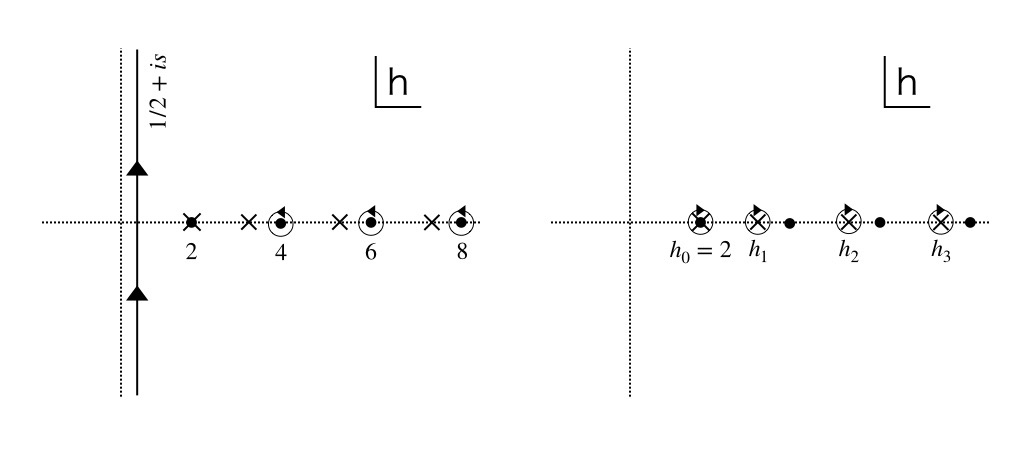
\includegraphics[width=11cm]{figures/poles}
	\caption{$h$平面における極。$h = 2n$における極を点、$k_c(h) = 1$となるような
	$h = h_m$における極をバツ印で表した。$h = 2 = h_0$では極が重なるため点とバツ印を重ねている。
	$h$の連続スペクトラム$h = 1/2 + is$の直線は
	右へずらす事ができ、点で表した$1/\tan(\pi h/2)$の極を相殺し、バツ印の極を選ぶ事になる。}
	\label{fig:poles}
\end{figure}

次に$\chi < 1$の場合について考える。
この場合は\eqref{eq:Psi_h_for_chi<1}式の${}_2F_1(1-h,1-h,2-2h,\chi)$を大きい$h > 0$に
持っていく事ができないため、少し回り道をする必要がある。
最初に、被積分関数の中の$\tan(\pi h/2)$を$\tan(\pi h)$に置き換えるために、
${}_2F_1$以外の残りの部分が持つ$h\to 1-h$の下での反対称性を利用する。
これによって$h\to 1-h$の下で対称となる被積分関数を得る。
この対称性を使って\eqref{eq:Psi_h_for_chi<1}式の$B$を$A$に置き換えれば、
\begin{align}
	\frac{\mathcal{F}_{h\neq 2}(\chi)}{\alpha_0}
	= \int &\frac{ds}{2\pi}\frac{h-1/2}{\pi\tan(\pi h/2)}
		\frac{k_c(h)}{1-k_c(h)}\frac{\Gamma(h)^2}{\Gamma(2h)}
		\chi^h\ {}_2F_1(h, h, 2h, \chi)\nonumber\\
	&+ \sum_{n=2}^{\infty}\mathrm{Res}\left[
		\frac{h-1/2}{\pi\tan(\pi h/2)}\frac{k_c(h)}{1-k_c(h)}\frac{\Gamma(h)^2}{\Gamma(2h)}
		\chi^h\ {}_2F_1(h, h, 2h, \chi)
	\right]_{h=2n}
\end{align}
という式に至る。
ここで留数の総和において、$h$が偶数の時
$\Psi_h(\chi) = \frac{\Gamma(h)^2}{\Gamma(2h)}\chi^h\ {}_2F_1(h, h, 2h, \chi)$
となる事を用いた。
この被積分関数は$\chi > 1$の場合のように右へずらす事が可能であり、選ぶべき留数が$k_c(h)=1$
となる$h = h_m$におけるものとなり、最終的に
\begin{align}
	\mathcal{F}_{h\neq 2} = -\alpha_0\sum_{m=0}^{\infty}\mathrm{Res}\left[
		\frac{h-1/2}{\pi\tan(\pi h/2)}\frac{k_c(h)}{1-k_c(h)}\frac{\Gamma(h)^2}{\Gamma(2h)}
		\chi^h\ {}_2F_1(h, h, 2h, \chi)
	\right]_{h=h_m}
	\hspace{5pt}\chi < 1
\end{align}
を得る。

\subsection{$h = 2$の場合の取り扱い}
$K_c$は固有値$k_c(h) = 1$を持つため、\eqref{eq:geometric_series_of_F}式の級数が発散する。
$k_c(h) = 1$となるのは$h = 2$における$SL(2, \mathbb{R})$のカシミール演算子$C_{1+2}$の固有関数である。
4点関数の有限な解を得るために、$K$を摂動的に共形極限から$\delta K$だけずらした場所でその固有関数を
扱う必要がある。
摂動による補正$\delta K$は、$K$を構成する2点関数$G$の非共形極限におけるリーディングオーダーでの補正
$\delta G$から生じる。
摂動パラメータは結合の大きさの逆数$(\beta J)^{-1}$である。

共形極限において、零温度と有限温度での両方の解$\eqref{eq:conformal_ansatz}$式は
$t$のリパラメトリゼーション不変性によって互いに等しいものであったが、摂動$\delta K$によって
共形対称性が破れるため、2つの解を等しいとする事はできない。
そこで最初から有限温度で議論し、周期を$\beta$から$2\pi$にするために
角度座標$\theta = 2\pi t / \beta$を導入する。値の範囲は$\theta \in [0, 2\pi]$である。
これは$\beta = 2\pi$と設定して議論を始めようとしているとも言える。
$\theta$は周期的ユークリッド時間である。

また$K$を直接論じるよりも、それを対称化した$\tilde{K}$の方が話を進めやすい。
\eqref{eq:symmetric_K}式で$t\to\theta$と変数変換すると
\begin{align}
	\tilde{K}(\theta_1, \theta_2; \theta_3, \theta_4)
	= -J^2(q-1)
		|G(\theta_{12})|^{\frac{q-2}{2}}
		G(\theta_{13})G(\theta_{24})
		|G(\theta_{34})|^{\frac{q-2}{2}}
	\label{eq:symmetric_K_in_theta}
\end{align}
となる。
またこの積分核$\tilde{K}$の反対称な固有関数を
\begin{align}
	\Psi_{h,n}^{\mathrm{exact}}(\theta_1, \theta_2)
	= - \Psi_{h,n}^{\mathrm{exact}}(\theta_2, \theta_1)
\end{align}
と書く事にする。
ここで添字$h$はあるラベルであり、後に詳しく説明する。
また$n$はフーリエ展開した際の$e^{-in(\theta_1 + \theta_2)/2}$の中の$n$である。
$\tilde{K}$は次式で与えられる内積において対称となる:
\begin{align}
	\innerprod{\Psi}{\Phi} \equiv
	\int_0^{2\pi}d\theta_1d\theta_2\ \Psi^*(\theta_1, \theta_2)\Phi(\theta_1, \theta_2).
	\label{eq:innerprod_in_finite_temp}
\end{align}

4点関数の表式を得るためには、輪を持たないラダーダイアグラム$\mathcal{F}_0$が
反対称単位行列
\begin{align}
	I(\theta_1, \cdots, \theta_4)
	= -\delta(\theta_{13})\delta(\theta_{24}) + \delta(\theta_{14})\delta(\theta_{23})
	= -2\sum_{h,n}\Psi_{h,n}^{\mathrm{exact}}(\theta_1, \theta_2)
		\Psi_{h,n}^{\mathrm{exact}*}(\theta_3, \theta_4)
\end{align}
に作用する$\tilde{K}$に比例するという事を用いると良い。
記号的には$\mathcal{F} = (1 - \tilde{K})^{-1}\tilde{K}\cdot I$の様に書き表す事ができ、
より正確には
\begin{align}
	\left[(q-1)J^2G(\theta_{12})^{\frac{q-2}{2}}G(\theta_{34})^{\frac{q-2}{2}}\right]
	\mathcal{F}(\theta_1,\cdots,\theta_2) = 
	2\sum_{h,n}\frac{k(h,n)}{1-k(h,n)}
		\Psi_{h,n}^{\mathrm{exact}}(\theta_1, \theta_2)
		\Psi_{h,n}^{\mathrm{exact}*}(\theta_3, \theta_4)
	\label{eq:fourpointfunc_in_theta}
\end{align}
となる。ここで$k(h,n)$は
固有関数$\Psi_{h,n}^{\mathrm{exact}}(\theta_1, \theta_2)$に対応する固有値である。
適切な固有関数の完全系の下で、この4点関数の表式はあらゆるカップリングの大きさ$\beta J$において正しい。

共形極限$\beta J \gg 1$に行くと、前節までの議論と接続できる。
固有関数$\Psi_{h,n}^{\mathrm{exact}}$は、
$SL(2,\mathbb{R})$に属する固有値$h(h-1)$を持つカシミール演算子$C_{1+2}$の固有関数$\Psi_{h,n}$となり、
固有関数も$k(h,n)\to k_c(h)$の様に$h$だけの関数になる。
また\eqref{eq:fourpointfunc_in_theta}式の$n$を走る総和は
($t$を$t = \tan\frac{\theta}{2}$によって円周上に射影した後で)
$\mathcal{F}_{h\neq 2}$の$\Psi_h$が現れる表式を与える。

4点関数の計算において$h = 2$からは無限大の寄与を得てしまう。
これはフーリエインデックス$n$について走る関数族$\Psi_{2,n}$によって与えられる。
この無限大を対処するには、共形極限から少し離れて共形対称性を破った上で
リーディングオーダーでの補正を求める必要がある。
特に共形極限での固有値$k_c(h)$への補正を計算する:
\begin{align}
	k(2, n) = 1 - O\left(\frac{1}{\beta J}\right).
\end{align}

\subsubsection{$\Psi_{2,n}$の具体型}
まず最初に$\Psi_{2,n}$の具体型を求める。
このためにリパラメトリゼーション不変性を活用する。
共形極限におけるシュウィンガー・ダイソン方程式\eqref{eq:conformalSD}式はリパラメトリゼーション不変性を持つ。
これによって$\theta\to\theta + \epsilon(\theta)$という様にリパラメトライズしたとすると
変化分$\delta_{\epsilon}G_c$は
\begin{align}
	\delta_{\epsilon}G_c
	= \left[\Delta\epsilon'(\theta_1) + \Delta\epsilon'(\theta_2)
		+ \epsilon(\theta_1)\frac{\partial}{\partial{\theta_1}}
		+ \epsilon(\theta_2)\frac{\partial}{\partial{\theta_2}}
	\right]G_c
	\label{eq:reparameterization_fomula}
\end{align}
となり、$G_c + \delta_{\epsilon}G_c$もまた\eqref{eq:conformalSD}式の解となる。
\eqref{eq:conformalSD}式の最初の式から
\begin{align}
	\delta_{\epsilon}G_c * \Sigma_c + G_c * \delta_{\epsilon}\Sigma_c = 0\hspace{5pt}
	\therefore\ 
	0 = \delta_{\epsilon}G_c + G_c * [(q-1)J^2G_c^{q-2}\delta_{\epsilon}G_c] * G_c
	= (1 - K_c)\delta_{\epsilon}G_c
	\label{eq:eigenfunc_of_Kc_is_reparametrization}
\end{align}
を得る。
ここで積$*$は
\begin{align}
	(F*G)(t_1, t_2) \equiv \int dt\ F(t_1, t)G(t, t_2)
\end{align}
を表す。
つまり変化分$\delta_{\epsilon}G_c$は$1 - K_c$を作用させる事により消滅する。
書き換えれば$K_c\delta_{\epsilon}G_c = \delta_{\epsilon}G_c$という固有値方程式になるため、
$\delta_{\epsilon}G_c$は固有値$1$を持つ$K_c$の固有関数である。
$\tilde{K}_c$において対応する固有関数は$|G_c|^{\frac{q-2}{2}}\delta_{\epsilon}G_c$である。

便利な基底を選ぶには$\epsilon \approx e^{-in\theta}$とすると良い。
\eqref{eq:conformal_ansatz}式の有限温度の$G_c$を\eqref{eq:reparameterization_fomula}式に代入し、
$|G_c|^{\frac{q-2}{2}}\delta_{\epsilon}G_c$を計算し、
最後に内積\eqref{eq:innerprod_in_finite_temp}式を用いて規格化すると、
$\tilde{K}_c$の固有値1の固有関数として
\begin{align}
	\Psi_{2,n} = \gamma_n\frac{e^{-iny}}{2\sin\frac{x}{2}}f_n(x),\hspace{20pt}
	f_n(x) = \frac{\sin\frac{nx}{2}}{\tan\frac{x}{2}} - n\cos\frac{nx}{2},
	\label{eq:eigenfunc_with_eigenvalue_1}
\end{align}
\begin{align}
	x = \theta_1 - \theta_2,\hspace{20pt}
	y = \frac{\theta_1 + \theta_2}{2},\hspace{20pt}
	\gamma_n^2 = \frac{3}{\pi^2|n|(n^2 - 1)}
	\label{eq:x_y_squaregamma}
\end{align}
を得る。
$\Psi_{2,n}$はカシミール演算子$C_{1+2}$の$h=2$の固有関数でもある。
また$n=-1,0,1$の場合、$G_c$の$SL(2,\mathbb{R})$共変性により
変化分$\delta_{\epsilon}G_c$は消滅する。
従って$|n| \geq 2$の場合のみ考えれば良い。
$n \geq 2$に対して、$\Psi_{2,n=2}$に$\hat{P}_1 + \hat{P}_2$を作用させる事により
全ての$\Psi_{2,n}$を得る事ができ、従って$SL(2,\mathbb{R})$のある表現を構成する。
$n \leq -2$の場合も同様である。

\subsubsection{固有値への補正}
ここでは$h=2$の固有値$k(2, n)$の共形極限での値$k_c(h=2)=1$に対する$(\beta J)^{-1}$補正を、
相互作用するフェルミオンの数$q$のラージ極限において計算する。
伝搬関数は\eqref{eq:firstOrder}式、また$g(\theta)$は\eqref{eq:explicit_g}式より与えられる。
ラダーダイアグラムの梯子のレールの部分の伝搬関数は
\begin{align}
	G(\theta) = \frac{1}{2}\sgn(\theta),
\end{align}
また輪の部分は($q$を偶数として)
\begin{align}
	G(\theta)^{q-2}
	= \frac{1}{2^{q-2}}\left(1 + \frac{g(\theta)}{q}\right)^{q-2}
	\to\ \frac{1}{2^{q-2}}e^{g(\theta)}
	\hspace{20pt}\mathrm{for}\ \ \ q \to \mathrm{large}
\end{align}
となる。
これらを用いると固有値方程式$\tilde{K}\Psi = k\Psi$は
\begin{align}
	-J^2q\int d\theta_1 d\theta_2\ 
		\frac{\sgn(\theta_{13})}{2}\frac{\sgn(\theta_{24})}{2}
		\frac{e^{(g(\theta_{12}) + g(\theta_{34}))/2}}{2^{q-2}}
		\Psi(\theta_1, \theta_2)
	= k\Psi(\theta_3, \theta_4)
\end{align}
と表される。
この固有値方程式の両辺に$\partial_{\theta_3}\partial_{\theta_4}e^{g(\theta_{34})/2}$を作用させ、
$\partial_x\sgn(x) = 2\delta(x)$を用いる積分を解消して微分方程式に直す事ができる。
\eqref{eq:explicit_g}式の$e^g$を代入し、固有値を$k = 2/h(h-1)$のようにパラメトライズし、
フーリエ変換した上で解くと
\begin{align}
	\Psi(\theta_1, \theta_2) = \frac{e^{-iny}}{\sin\frac{\tilde{x}}{2}}\psi_n)(x),
	\hspace{20pt}\tilde{x} = vx + (1-v)\pi,
	\label{eq:eigenfunc_of_tilde_K}
\end{align}
\begin{align}
	\left(
		n^2 + 4\frac{\partial^2}{\partial x^2} - 
		\frac{h(h-1)v^2}{\sin^2\frac{\tilde{x}}{2}}
	\right)\psi_n(x) = 0
	\label{eq:diffeq_for_large_q}
\end{align}
という解を得る。ここで$v$は\eqref{eq:explicit_g}式の2つ目の式によって定義される。
$x$と$y$は\eqref{eq:x_y_squaregamma}式で与えられる。
$v=1$の時は$\beta \mathcal{J} \to \infty$であり、\eqref{eq:diffeq_for_large_q}式は
共形変換群$SL(2,\mathbb{R})$のカシミール演算子$C_{1+2}$の固有関数を与える方程式となる。
ここで$\mathcal{J}$は\eqref{eq:diffeq_for_g}式の2つ目の式で与えられる、ラージ$q$で
一定となるようにリスケールされた相互作用の大きさである。
しかし\eqref{eq:diffeq_for_large_q}式は任意の$\beta \mathcal{J}$に対して
ラージ$q$の固有関数を与える。

探したいものは然るべき対称性を備えた固有関数である。
4点関数は$\theta_1, \theta_2$の2変数関数として
\begin{align}
	F(\theta_1, \theta_2) = -F(\theta_2, \theta_1),\hspace{10pt}
	F(\theta_1 + 2\pi, \theta_2) = -F(\theta_1, \theta_2),\hspace{10pt}
	F(\theta_1, \theta_2 + 2\pi) = -F(\theta_1, \theta_2)
	\label{eq:properties_of_fourpointfunc}
\end{align}
という性質を持つ。最初の2つの性質は1つにまとめる事ができ、それを$x$と$y$を使って表すと
\begin{align}
	F(x, y) = F(2\pi - x, y + \pi)
\end{align}
というものになる。
また\eqref{eq:properties_of_fourpointfunc}式の最初の性質より$x > 0$と制限できる。
さらに\eqref{eq:eigenfunc_of_tilde_K}式の$e^{-iny}$の存在により、
$\psi_n(x)$は$x=\pi$で、$n$が偶数の時は対称、奇数の時は反対称となる必要がある。
以上を踏まえると$\psi_{h,n}$は、$\tilde{n} = n/v$として、
\begin{align}
	\psi_{h,n}(x)
	\approx \left(\sin\frac{\tilde{x}}{2}\right)^h\ 
	{}_2F_1\left(
		\frac{h-\tilde{n}}{2}, \frac{h+\tilde{n}}{2},
		\frac{1}{2},\cos^2\frac{\tilde{x}}{2}
		\right)\hspace{85pt}(n\ \ \mathrm{even})
	\label{eq:psi_hn_for_even}
\end{align}
\begin{align}
	\psi_{h,n}(x)
	\approx \cos\frac{\tilde{x}}{2}\left(\sin\frac{\tilde{x}}{2}\right)^h\ 
		{}_2F_1\left(
			\frac{1 + h - \tilde{n}}{2},
			\frac{1 + h + \tilde{n}}{2},
			\frac{3}{2},
			\cos^2\frac{\tilde{x}}{2}
		\right)\hspace{30pt}(n\ \ \mathrm{odd})
	\label{eq:psi_hn_for_odd}
\end{align}
となる。$\psi$は$x=0$で消滅するという境界条件によって$h$の量子化条件が決まる。

欲しい固有関数は強結合領域で$h=2$共形固有関数になるものである。
$h\approx 2$の時、$\tilde{x}\approx 0$発散する。
$(1-v)$の2次のオーダーにおいて、この発散が存在しないための条件は
超幾何関数の1番目か2番目の変数の少なくともどちらかが負の整数になるというものである。
2に近い解は$h_n = 2 + |\tilde{n}| - |n| = 2 + |n|\frac{1-v}{v}$となる。
\eqref{eq:eigenvalue_of_Kc}式から$q = \infty$の時$k_c(h) = \frac{2}{h(h-1)}$
であるのを思い出せば、これを展開して
\begin{align}
	k(2, n)
	= 1 - \frac{3|n|}{2}(1 - v) + \left(\frac{7n^2}{4} - \frac{3|n|}{2}\right)(1 - v)^2
		+ \cdots
	= 1 - \frac{3|n|}{\beta \mathcal{J}} + \frac{7n^2}{(\beta \mathcal{J})^2} + \cdots
	\label{eq:eigenvalue_at_large_q}
\end{align}
を得る。
ここで最後の表式は$v$を\eqref{eq:explicit_g}式の右の式から$(\beta \mathcal{J})^{-1}$
で展開したものを用いた:
\begin{align}
	1 - v = \frac{2}{\beta\mathcal{J}} - \frac{4}{(\beta\mathcal{J})^2} + \cdots.
\end{align}

次に一般の$q$について考える。
固有値方程式$\tilde{K} \Psi_{2,n} = k(2, n)\Psi_{2,n}$を厳密に解く事はできないが、
$\tilde{K} = \tilde{K}_c + \delta\tilde{K}$として共形極限からの摂動論を1次まで
計算する事は可能である。
計算するべきは$\innerprod{\Psi_{2,n}}{\delta\tilde{K}\cdot\Psi_{2,n}}$となる。

摂動補正$\delta\tilde{K}$は共形伝搬関数に摂動を加えた$G_c + \delta G$というものを
$\tilde{K}_c$の表式\eqref{eq:symmetric_K_in_theta}式に代入する事で得られる。
ここでラージ$q$に戻って$\delta G$を求めると、\eqref{eq:conformal_ansatz}式と
\eqref{eq:explicit_g}式から有限温度のラージ$q$共形伝搬関数は
\begin{align}
	G(\theta) = G_c(\theta)\left[
		1 - \frac{2}{q}\frac{1}{\beta\mathcal{J}}
		\left(2 + \frac{\pi - \theta}{\tan\frac{\theta}{2}}\right) + \cdots
	\right]
\end{align}
となるので、$(\beta\mathcal{J})^{-1}$補正$\delta G$は
\begin{align}
	f_0(\theta) \equiv 2 + \frac{\pi - \theta}{\tan\frac{\theta}{2}}
	\label{eq:f_0}
\end{align}
に比例する事がわかる。
これは\eqref{eq:eigenfunc_with_eigenvalue_1}式の$f_n$で$n\to 0$としたものに一致する。
\eqref{eq:f_0}式を用いて一般の$q$における$G_c$への補正は
\begin{align}
	\frac{\delta G}{G_c} = -\frac{\alpha_G}{\beta\mathcal{J}}f_0
	\label{eq:perturbation_correction_for_Gc}
\end{align}
のように表せるはずである。
ここで$\alpha_G$は$q\to\infty$で$q\alpha_G\to 2$となるような係数である。
数値解析によって\eqref{eq:perturbation_correction_for_Gc}式は
様々な$q$の値において精度の良いフィッティング関数となる事が示されている\cite{maldacena}。

固有値への補正項を求めるために直接$\innerprod{\Psi_{2,n}}{\delta\tilde{K}\cdot\Psi_{2,n}}$
を計算しても良いが、手っ取り早い方法が存在し、
\begin{align}
	\frac{1}{q\alpha_G}\frac{\innerprod{\Psi_{h,n}}{\tilde{K}\cdot\Psi_{2,n}}}{1-k_c(h)}
\end{align}
が実は$q$に依らない量である事を用いる\cite{maldacena}。
この量は$h=2$で極を持ち、その留数は固有値への補正項に比例する。
この留数とラージ$q$における固有値の表式\eqref{eq:eigenvalue_at_large_q}式、
及びラージ$q$において成り立つ性質
($q\alpha_G = 2,\ k'_c(2) = -3/2$)を用いると、一般の$q$における固有値
\begin{align}
	k(2, n) &= 1 - \frac{\alpha_K}{\beta\mathcal{J}}|n| + \cdots\\
	\alpha_K &\equiv -qk'_c(2)\alpha_G
		= \left[
			\frac{\pi q}{\sin\frac{2\pi}{q}} + \frac{q^3(6-q) - 6q^2}{2(q-1)(q-2)}
		\right]\alpha_G
	\label{eq:corrected_eigenvalue}
\end{align}
を得る。
$\alpha_K$は\eqref{eq:eigenvalue_at_large_q}式よりラージ$q$で3となる係数である。
$\alpha_K$を$q$に関して数値的に求めると、どの$q$に対しても3に近い事がわかる\cite{maldacena}。

\subsubsection{$h = 2$の4点関数への寄与}
ここまでの議論により4点関数\eqref{eq:fourpointfunc_in_theta}式での発散は
共形極限から少しずれる事によって処理されたので、$h=2$の4点関数への寄与は有限となり、
$\beta\mathcal{J}$のオーダーの値を持つ。
ただし$h=2$の寄与はこれだけではなく、$\frac{k(2,n)}{1-k(2,n)}$による$(\beta\mathcal{J})^0$の
寄与も存在する。
ここでは先に$O(\beta\mathcal{J})$の大きさの寄与を計算し、
$O(1)$の寄与の計算は後で$q=\infty$において計算する。

具体的に計算すれば、$h=2$の$O(\beta\mathcal{J})$の寄与は
\begin{align}
	\frac{\mathcal{F}_{\mathrm{big}}(\theta_1,\cdots,\theta_4)}{G(\theta_{12})G(\theta_{34})}
	= \frac{6\alpha_0}{\pi^2\alpha_K}\beta\mathcal{J}\sum_{|n|\geq 2}
		\frac{e^{in(y' - y)}}{n^2(n^2 - 1)}
		\left[
			\frac{\sin\frac{nx}{2}}{\tan\frac{x}{2}} - n\cos\frac{nx}{2}
		\right]
		\left[
			\frac{\sin\frac{nx'}{2}}{\tan\frac{x'}{2}} - n\cos\frac{nx'}{2}
		\right],
	\label{eq:F_big}
\end{align}
\begin{align}
	x = \theta_{12},\hspace{20pt}
	\tilde{x} = \theta_{34},\hspace{20pt}
	y = \frac{\theta_1 + \theta_2}{2},\hspace{20pt}
	y' = \frac{\theta_3 + \theta_4}{2}
\end{align}
となる。
さらに共形極限において\eqref{eq:eigenfunc_of_Kc_is_reparametrization}式から
$h=2$の固有関数はリパラメトリゼーション$\theta\to\theta + \epsilon(\theta)$
による変化分$\delta_{\epsilon}G$そのものであった事から、特に$\epsilon_n \propto e^{-in\theta}$
として
\begin{align}
	\mathcal{F}_{\mathrm{big}} = 
	\sum_n \average{\epsilon_n\epsilon_{-n}}\delta_{\epsilon_n}G\delta_{\epsilon_{-n}}G,
	\hspace{20pt}
	\average{\epsilon_n\epsilon_{-n}} = 
	\left(\frac{6\alpha_0q^2}{\alpha_K N}\right)\frac{\beta\mathcal{J}}{n^2(n^2-1)}
\end{align}
と書く事ができる。
$\average{\epsilon_n\epsilon_{-n}}$はフーリエ変換によって
\begin{align}
	\average{\epsilon(\theta)\epsilon(0)}
	= \frac{1}{N}\frac{6(\beta\mathcal{J}) \beta^2 q^2 \alpha_0}{(2\pi)^4 \alpha_K}
	\left[
		-\frac{1}{2}(|\theta| - \pi)^2 + (|\theta| - \pi)\sin|\theta
		+ 1 + \frac{\pi^2}{6} + \frac{5}{2}\cos\theta
	\right]
	\label{eq:propagator_of_epsilon}
\end{align}
と変換される。
\eqref{eq:F_big}式の$n$を走る和はこの2点関数と
リパラメトリゼーション\eqref{eq:reparameterization_fomula}式を用いる事によって計算できる。
結果は4つのフェルミオンの順番によって変わり、
$\average{\psi_i\psi_i\psi_j\psi_j}$か$\average{\psi_i\psi_j\psi_i\psi_j}$かで場合分け
する必要がある。

最初の$iijj$という順番の場合は
\begin{align}
	iijj\ \ \mathrm{order:}\hspace{20pt}
	\frac{\mathcal{F}_{\mathrm{big}}(\theta_1, \cdots, \theta_4)}{G(\theta_{12})G(\pi)}
	= \frac{6\alpha_0}{\pi^2\alpha_K}\beta\mathcal{J}
		\left(
			\frac{\theta_{12}}{2\tan\frac{\theta_{12}}{2}} - 1
		\right)
		\left(
			\frac{\theta_{34}}{2\tan\frac{\theta_{34}}{2}} - 1
		\right)
	\label{eq:h_2_contribution_in_iijj_order}
\end{align}
で与えられる。また$ijij$という順番の場合は、特に$\theta_3 = 0, \theta_4 = \pi$とすると
結果が簡略化される:
\begin{align}
	ijij\ \ \mathrm{order:}\hspace{20pt}
	\frac{\mathcal{F}_{\mathrm{big}}(\theta_1, \theta_2, 0, \pi)}{G(\theta_{12})G(\pi)}
	= - \frac{6\alpha_0}{\pi^2\alpha_K}\beta\mathcal{J}
		\left(
			\frac{\theta_{12}}{2\tan\frac{\theta_{12}}{2}} - 1
			- \pi \frac{\sin\frac{\theta_1}{2}\sin\frac{\theta_2}{2}}{|\sin\frac{\theta_{12}}{2}|}
		\right).
	\label{eq:h_2_contribution_in_ijij_order}
\end{align}

\subsubsection{$q=\infty$における$h=2$の寄与}
次に$h=2$の$O((\beta\mathcal{J})^0)$の寄与をラージ$q$において計算する。
ラージ$q$ではラダーダイアグラムの梯子のレールの伝搬関数は$\sgn(\theta)$に比例するため、
$K$は次式のような微分演算子のグリーン関数となる事が示せる:
\begin{align}
	-\frac{2}{v^2\tilde{P}^2}\pdiff{\theta_1}\pdiff{\theta_2}K(\theta_1, \cdots, \theta_4)
	= \delta(\theta_{13})\delta(\theta_{24}),\hspace{20pt}
	\tilde{P} = \frac{1}{\sin\frac{\tilde{x}}{2}},\hspace{20pt}
	\tilde{x} = vx + (1 - v)\pi.
\end{align}

4点関数は$\mathcal{F} = (K^{-1} - 1)^{-1}$の様に書けるため、両辺に$(K^{-1} - 1)$を作用させれば
$\mathcal{F}$の満たす微分方程式を得る。
この際、$x = \theta_{12}, y = \frac{\theta_1 + \theta_2}{2}$という座標を導入すると便利である。
ただしこの$x$と$y$は配位を足しすぎてしまうため、$x \geq 0, \tilde{x} \geq 0, y \geq y'$
という様に制限する必要がある。
$\mathcal{F}$の満たす微分方程式は
\begin{align}
	\left(
		- \frac{1}{4}\frac{\partial^2}{\partial y^2}
		+ v^2\frac{\partial^2}{\partial \tilde{x}^2}
		- \frac{v^2\tilde{P}^2}{2}
	\right)\mathcal{F}(x, y, x', y')
	= \delta(y - y')\delta(x - x') + \delta(y - y' - \pi)\delta(2\pi - x - x')
\end{align}
となる。
この微分方程式は変数分離法によって解く事が可能である。
まず$-\partial^2_{\tilde{x}} + \tilde{P}^2 / 2$の固有関数による完全系で展開する。
ただし境界条件は$x = 0$で0とする。
この固有関数は\eqref{eq:psi_hn_for_even}式や\eqref{eq:psi_hn_for_odd}式で
$h=2$としたものに一致し、
\eqref{eq:eigenfunc_with_eigenvalue_1}式で定義されている$f_n$に簡略化される。
固有値は$n^2/4$である。
$f_n$は完全系の条件
\begin{align}
	\sum_{n>2}\frac{f_n(\tilde{x})f_n(\tilde{x}')}{\pi(n^2 - 1)}
	= \delta(\tilde{x} - \tilde{x}'),\hspace{20pt}
	\sum_{n>2}(-1)^n\frac{f_n(\tilde{x})f_n(\tilde{x}')}{\pi(n^2 - 1)}
	= \delta(2\pi - \tilde{x} - \tilde{x}')
\end{align}
を満たす事から、$\mathcal{F}$は
\begin{align}
	\mathcal{F}(x, y, x', y')
	= \sum_{n>2}H_n(y - y')\frac{f_n(\tilde{x})f_n(\tilde{x}')}{\pi(n^2 - 1)},
	\label{eq:h2_contribution_for_fourpointfunc_in_large_q}
\end{align}
\begin{align}
	\left(-\frac{1}{4}\frac{\partial^2}{\partial y^2} - \frac{v^2n^2}{4}\right)H_n(y)
	= v[\delta(y) + (-1)^n\delta(y-\pi)]
\end{align}
となる。
$H_n$は周期$2\pi$の連続関数だが、$y=0, \pi$で一階導関数は不連続である。
$y=0$における不連続性は$0^+$や$2\pi^-$における導関数の不連続性と同じである。
これらの条件を解くと、$0 < y < 2\pi$の範囲で
\begin{align}
	H_n(y)
	&= -\frac{2}{n\sin(n\pi v)}
	\left(
		\cos[nv(y - \pi)] + (-1)^n\cos[nv(|y-\pi| - \pi)]
	\right)\\
	&= \frac{4\cos(ny)}{\pi n^2(1-v)}
		+ \frac{4(y-\frac{\pi}{2})\sin(ny)}{\pi n} + O(1 - v)\\
	&= \left(
			\frac{\beta\mathcal{J}}{2} + 1 - \left(y - \frac{\pi}{2}\pdiff{y}\right)	
		\right)\frac{4\cos(ny)}{\pi n^2} + O\left(\frac{1}{\beta\mathcal{J}}\right)
\end{align}
という結果になる。
2行目では$0 < y < \pi$と仮定して$(1 - v)$で展開した。
$\pi < y < 2\pi$ならば$\pi / 2$を$3\pi / 2$に置き換えれば良い。
また3行目では$(1-v)^{-1}\approx \beta\mathcal{J}/2 + 1$を用いた。
この3行目の式を\eqref{eq:h2_contribution_for_fourpointfunc_in_large_q}式に代入し、
\begin{align}
	f_n(\tilde{x}) = f_n(x) + (1-v)(\pi - x)\frac{d}{dx}f_n(x) + \cdots
\end{align}
を用いて展開すると、ラージ$q$における4点関数として
\begin{align}
	\mathcal{F}(x, y, x', 0)
	= \left[
		\beta\mathcal{J} - 2\left\{-1 + \left(y - \frac{\pi}{2}\right)\pdiff{y}
		+ (x-\pi)\pdiff{x} + (x' - \pi)\pdiff{x'}\right\}
	\right]\nonumber\\
	\times \sum_{|n|\geq 2} \frac{e^{-iny}f_n(x)f_n(x')}{\pi^2n^2(n^2-1)}
	\label{eq:fourpointfunc_in_large_q_upto_order1}
\end{align}
を得る。
$O(\beta\mathcal{J})$の項は\eqref{eq:F_big}式の$\mathcal{F}_{\mathrm{big}}$で
ラージ$q$極限を取ったものに一致する($\alpha_0=2, \alpha_K=3, G=1/2$)。

\subsection{4点関数: 最終結果}
一般の$q$について伝搬関数に補正$\delta G$を加えると、
4点関数は\eqref{eq:fourpointfunc_in_theta}式より次のような補正を受ける:
\begin{align}
	\frac{\mathcal{F}(\theta_1, \cdots, \theta_4)}{G(\theta_{12})G(\theta_{34})}
	&\supset -\frac{q}{2}
		\left[
			\frac{\delta G(\theta_{12})}{G_c(\theta_{12})}
			+ \frac{\delta G(\theta_{34})}{G_c(\theta_{34})}
		\right]
		\frac{\mathcal{F}_{\mathrm{big}}(\theta_1, \cdots, \theta_4)}
			{G_c(\theta_{12})G_c(\theta_{34})}\\
	&= \frac{3\alpha_0}{\pi^2|k'_c(2)|}[f_0(\theta_{12}) + f_0(\theta_{34})]
		\sum_{|n|\geq 2}\frac{e^{in(y'-y)}f_n(x)f_n(x')}{n^2(n^2-1)}.
\end{align}
ここで重要な点は、この補正項は$\alpha_0 / k'_c(2)$という因子を通してのみ$q$に依存している事である。
従ってラージ$q$における4点関数の結果\eqref{eq:fourpointfunc_in_large_q_upto_order1}式を
一般の$q$に対する$\mathcal{F}$に使う事が可能である。
$\chi < 1$の時は
\begin{align}
	&\frac{\mathcal{F}(x,y,x',0)}{G(x)G(x')}\nonumber\\
	&= \alpha_0\left\{
		\frac{6\beta\mathcal{J}}{\alpha_K} - \frac{6}{|k'_c(2)|}
		\left[
			-1 + \left(y-\frac{\pi}{2}\right)\pdiff{y}
			+ (x - \pi)\pdiff{x} + (x' - \pi)\pdiff{x'}
		\right]
	\right\}\sum_{|n|\geq 2}\frac{e^{-iny}f_n(x)f_n(x')}{\pi^2n^2(n^2-1)}\nonumber\\
	&\hspace{20pt}
	-\alpha_0\sum_{m=1}^{\infty}\mathrm{Res}\left[
		\frac{h-1/2}{\pi\tan(\pi h/2)}\frac{k_c(h)}{1-k_c(h)}\frac{\Gamma(h)^2}{\Gamma(2h)}
		\chi^h\ {}_2F_1(h, h, 2h, \chi)
	\right]_{h=h_m}
	\hspace{20pt}\chi < 1
\end{align}
となる。
$\chi > 1$に関しては
$\frac{\Gamma(h)^2}{\Gamma(2h)}\chi^h\ {}_2F_1(h, h, 2h, \chi)\to \Psi_h(\chi)$
という置き換えをすると得る事ができる。

\pagebreak

	\section{量子カオス}


\pagebreak

	\section{ランダム行列理論}


\pagebreak

	\section{カオスとしてのSYK模型}


\pagebreak

	\section{終わりに}


\pagebreak

	\appendix
	\section{有効作用の計算 \label{app:effective_action}}
	\renewcommand{\theequation}{A.\arabic{equation} }
	\setcounter{equation}{0}

	SYK模型のラグランジアンは
	\begin{align}
	L = \frac{1}{2}\sum_{i = 1}^{N} \psi_i \deriv \psi_i
		- \frac{1}{4!} \sum_{i,j,k,l = 1}^{N} J_{ijkl} \psi_i\psi_j\psi_k\psi_l
	\label{eq:laglangian}
	\end{align}
	で与えられる。
	SYK模型ではしばしば有限温度を考慮するため、分配関数はユークリッド化したものを計算する:
	\begin{align}
	Z = \pathint{\psi} \exp\left(- \int dt\  L\right).
	\label{eq:partition}
	\end{align}
	以下では\eqref{eq:partition}式を乱数$J_{ijkl}$について平均を取るという
	disorder-averageの計算を行い、その後フェルミオンについて積分し有効作用を得る事を目標とする。

	disorder-averageは
	\begin{align}
	\average{Z} = \int \prod_{i<j<k<l}^{N}\left[dJ_{ijkl}\ P(J_{ijkl})\right]Z
	\end{align}
	を計算すれば良い。
	以下では表記を簡潔にするために
	\begin{align}
	a &\equiv \frac{N^3}{12J^2}\\
	I_{ijkl} &\equiv \int dt\ \psi_i\psi_j\psi_k\psi_l
	\end{align}
	としておく。
	$J_{ijkl}$についての積分が実行される部分が明確になるように式変形すると
	\begin{align}
	\average{Z} =
		\pathint{\psi} &\exp\left(- \int dt\ \sum_i \frac{1}{2}\psi_i\deriv\psi_i\right)
		\nonumber\\
		&\times \underbrace{\int \left[\prod_{i<j<k<l}
			dJ_{ijkl}\ \sqrt{\frac{a}{\pi}} \exp\left(-aJ_{ijkl}^{\, 2}\right)
			\right]
			\exp\left(\frac{1}{4!}\sum_{i,j,k,l}I_{ijkl}J_{ijkl}\right)}_{\equiv G}
	\end{align}
	となる。ここから更に$G$を複数のガウス積分の積となるように変形すると
	\begin{align}
	G = \left(\frac{a}{\pi}\right)^{4!\combination{N}{4} / 2}
		\prod_{i<j<k<l}\int dJ_{ijkl}\ \exp\left(
		-aJ_{ijkl}^{\, 2} + I_{ijkl}J_{ijkl}
		\right)
	\end{align}
	となる。
	ここで$J_{ijkl}$と$I_{ijkl}$が反対称テンソルである事を用いて
	\begin{align}
	\frac{1}{4!}\sum_{i,j,k,l}I_{ijkl}J_{ijkl} = \sum_{i<j<k<l}I_{ijkl}J_{ijkl}
	\end{align}
	を使用した。
	あとは通常のガウス積分を実行すると
	\begin{align}
	G = \exp\left(\frac{3J^2}{N^3}\sum_{i<j<k<l}I_{ijkl}^{\, 2}\right)
	  = \exp\left(\frac{3J^2}{4!N^3}\sum_{i,j,k,l}I_{ijkl}^{\, 2}\right)
	\end{align}
	となり、
	\begin{align}
	\average{Z} = \pathint{\psi} &\exp\left(
	- \int dt\ \sum_i \frac{1}{2}\psi_i\deriv\psi_i \right. \nonumber\\
	&\left.
	+ \frac{3J^2}{4!N^3}\sum_{i,j,k,l}\int dt_1dt_2\
		\psi_i(t_1)\psi_j(t_1)\psi_k(t_1)\psi_l(t_1)
		\psi_i(t_2)\psi_j(t_2)\psi_k(t_2)\psi_l(t_2)
	\right)
	\end{align}
	という結果を得る。
	次はフェルミオンについて積分するのであるが、その前に
	\begin{align}
	G(t_1, t_2) = \frac{1}{N}\sum_{i = 1}^{N}\psi_i(t_1)\psi_i(t_2)
	\end{align}
	という場を導入するために
	\begin{align}
	1 &= \pathint{G}\delta\left(NG - \sum_i\psi_i\psi_i\right)\nonumber\\
	  &= \pathint{G}\pathint{\Sigma}\exp\left(
	  		-\int dt_1dt_2\ \frac{1}{2}\Sigma(t_1, t_2)\left(
	  		NG(t_1, t_2) - \sum_i\psi_i(t_1)\psi_i(t_2)\right)
	  	\right)
	\end{align}
	を$\average{Z}$に挿入する\footnote{ディラックのデルタ関数をフーリエ変換したものはもちろん
	\begin{align}
	\delta(x) \propto \int dp\ \exp(ipx)\nonumber
	\end{align}であるが、今は$\Sigma(t_1, t_2)$を虚軸方向に積分していると考えているため、
	結果として虚数単位$i$がさらに$i$倍され負号となる。}。
	この時、挿入したデルタ関数によって
	\begin{align}
	\sum_{i,j,k,l}\int dt_1dt_2\
	\psi_i(t_1)\psi_j(t_1)\psi_k(t_1)\psi_l(t_1)
	\psi_i(t_2)\psi_j(t_2)\psi_k(t_2)\psi_l(t_2)
	\to N^4\int dt_1 dt_2 G(t_1, t_2)^4
	\end{align}
	という置き換えができる。
	以上を踏まえてフェルミオンの積分が実行される部分が明確になるように式変形を行うと
	\begin{align}
	\average{Z} = \pathint{G}\pathint{\Sigma}&\exp\left(
	-\frac{N}{2}\int dt_1dt_2\ \left(\Sigma G - \frac{J^2}{4}G^4\right)
	\right)\nonumber\\
	&\times\underbrace{\pathint{\psi}\exp\left(
	-\sum_i\int dt_1dt_2\ \frac{1}{2}\psi_i(t_1)\left(
	\delta(t_1 - t_2)\frac{d}{dt_1} - \Sigma(t_1, t_2)
	\right)\psi_i(t_2)
	\right)}_{\equiv F}
	\end{align}
	となる。
	あとは$F$と置いた部分を計算するのだが、そのためには次の公式を使うとよい\cite{haber}:
	\begin{align}
	\int d\theta \exp\left(-\frac{1}{2}\theta\cdot M\cdot\theta\right) = \sqrt{\det(M)}
	\end{align}
	ここで$\theta = (\theta_1, \cdots, \theta_n)$は$n$個のグラスマン数であり、$M$は反対称行列である。
	これを用いて、
	\begin{align}
	F &= \prod_i \pathint{\psi_i} \exp\left(
	-\int dt_1dt_2\ \frac{1}{2}\psi_i(t_1)\left(
	\delta(t_1 - t_2)\frac{d}{dt_1} - \Sigma(t_1, t_2)
	\right)\psi_i(t_2)\right)\nonumber\\
	&= \prod_i \left[
	\det\left(\delta(t_1 - t_2)\frac{d}{dt_1} - \Sigma(t_1 - t_2)\right)
	\right]^{1/2}\nonumber\\
	&= \left[\det\left(\deriv - \Sigma\right)\right]^{N/2}\nonumber\\
	&= \exp\left(\frac{N}{2}\log\det\left(\deriv - \Sigma\right)\right)
	\end{align}
	となる。ここで
	\begin{align}
	\delta(t_1 - t_2)\frac{d}{dt_1} - \Sigma(t_1 - t_2) \to \deriv - \Sigma
	\end{align}
	という記号的な処理を施した。

	以上より
	\begin{align}
	\average{Z} &= \pathint{G}\pathint{\Sigma}
		\exp\left(
		\frac{N}{2}\log\det\left(\deriv - \Sigma\right)
		- \frac{N}{2}\int dt_1dt_2\ \left(\Sigma G - \frac{J^2}{4}G^4\right)
		\right)\nonumber\\
	&\equiv \pathint{G}\pathint{\Sigma}\exp(-I_{\mathrm eff})
	\end{align}
	となり、有効作用として
	\begin{align}
	\frac{I_{\mathrm eff}}{N} =
		- \frac{1}{2}\log\det\left(\deriv - \Sigma\right)
		+ \frac{1}{2}\int dt_1dt_2\ \left(\Sigma G - \frac{J^2}{4}G^4\right)
	\end{align}
	を得た。

	\pagebreak

	\section{係数$b$の計算 \label{app:b}}
	\renewcommand{\theequation}{B.\arabic{equation}}
	\setcounter{equation}{0}
	
	この付録では\eqref{eq:conformal_ansatz}式の係数$b$の計算方法について述べる.
	まず\eqref{eq:conformalSD}式の2つの式を一つにまとめると
	\begin{align}
		J^2\int ds\ G(s - t_1)G(s - t_2)^{q - 1} = -\delta(t_2 - t_1)
		\label{eq:intOfGG}
	\end{align}
	となる.この積分を実行するには、
	\begin{align}
	\frac{\sgn(t)}{|t|^{2\Delta}} = 
		\int \frac{d\omega}{2\pi}\exp(-i\omega t)\ 
		i\, 2^{1 - 2\Delta}\sqrt{\pi}\frac{\Gamma(1 - \Delta)}{\Gamma(1/2 + \Delta)}
		|\omega|^{2\Delta - 1}\sgn(\omega)
	\end{align}
	を使用すると便利である.
	少しの計算のあとに、
	\begin{align}
	-\delta(t) = &-J^2b^q\pi
		\frac{\Gamma(1 - \Delta)\Gamma(\Delta)}{\Gamma(1/2 + \Delta)\Gamma(3/2 - \Delta)}
		\nonumber\\
		&\times \int ds\ 
		\int \frac{d\omega}{2\pi}\ \exp(-i\omega(t - s))\ |\omega|^{2\Delta - 1}\sgn(\omega)
		\int \frac{d\Omega}{2\pi}\ \exp(-i\Omega s)\ |\Omega|^{1 - 2\Delta}\sgn(\Omega)
	\end{align}
	という式にたどり着く。
	積分の部分は最初に$s$について実行すると$\delta(\omega - \Omega)$が現れ、その後
	$\omega$および$\Omega$で積分すると$\delta(t)$が現れる。
	またガンマ関数の部分については
	\begin{align}
	\Gamma(z)\Gamma(1 - z) = \frac{\pi}{\sin(\pi z)}
	\hspace{30pt}
	{\rm for}\ {}^{\forall}z \notin \mathbb{Z}
	\end{align}
	という性質と$\Gamma(1 + z)\Gamma(z) = z\Gamma(z)$を用いることで
	\begin{align}
	\frac{\Gamma(1 - \Delta)\Gamma(\Delta)}{\Gamma(1/2 + \Delta)\Gamma(3/2 - \Delta)}
	= \frac{1}{(1/2 - \Delta) \tan(\pi\Delta)}
	\end{align}
	となる. 以上より、係数$b$は
	\begin{align}
		J^2b^q\pi = \left(\frac{1}{2} - \Delta\right)\tan(\pi\Delta)
	\end{align}
	という式により決定できる。
	
	\pagebreak
	\begin{thebibliography}{99}
%	\bibitem{maldacena}
%		J. Maldacena and D. Stanford,
%		"Comments on the Sachdev-Ye-Kitaev model,"
%		\href{https://arxiv.org/pdf/1604.07818.pdf}{arXiv:1604.07818 [hep-th]}
%	\bibitem{rosenhaus}
%		V. Rosenhaus,
%		"An introduction to the SYK model,"
%		\href{https://arxiv.org/pdf/1807.03334.pdf}{arXiv:1807.03334v1 [hep-th]}
%	\bibitem{polchinski}
%		J. Polchinski and V. Rosenhaus,
%		"The Spectrum im the Sachdev-Ye-Kitaev Model,"
%		\href{https://arxiv.org/pdf/1601.06768.pdf}{arXiv:1601.06768 [hep-th]}
%	\bibitem{gross}
%		D. J. Gross and V. Rosenhaus,
%		"A Generalization of Sachdev-Ye-Kitaev,"
%		\href{https://arxiv.org/pdf/1610.01569.pdf}{arXiv:1610.01569 [hep-th]}
%	\bibitem{shenker}
%		J. Maldacena, S. H. Shenker and D. Stanford,
%		"A bound on chaos,"
%		\href{https://arxiv.org/pdf/1503.01409.pdf}{arXiv:1503.01409 [hep-th]}
%	\bibitem{liu}
%		J. Liu,
%		"Spectral form factors and late time quantum chaos,"
%		\href{https://arxiv.org/pdf/1806.05316.pdf}{arXiv:1806.05316 [hep-th]}
%	\bibitem{polchinski_chaos}
%		J. S. Cotler, G. Gur-Ari, M. Hanada, J. Polchinski, P. Saad, S. H. Shenker,
%		D. Stanford, A. Streicher and M. Tezuka,
%		"Black Holes and Random Matrices,"
%		\href{https://arxiv.org/pdf/1611.04650.pdf}{arXiv:1611.04650 [hep-th]}
%	\bibitem{stanford_chaos}
%		P. Saad, S. H. Shenker and D. Stanford,
%		"A semiclassical ramp in SYK and in gravity,"
%		\href{https://arxiv.org/pdf/1806.06840.pdf}{arXiv:1806.04650 [hep-th]}
%	\bibitem{haber}
%	H. E. Haber,
%	\href{http://scipp.ucsc.edu/~haber/webpage/pfaffian2.pdf}{"Notes on antisymmetric matrices and the pfaffian"}
%	\bibitem{tarnopolsky}
%		G. Tarnopolsky,
%		"On large $q$ expansion in the Sachdev-Ye-Kitaev model,"
%		\href{https://arxiv.org/pdf/1801.06871.pdf}{arXiv:1801.06871 [hep-th]}
%	\bibitem{andrzejewski}
%		K. Andrzejewski,
%		"Quantum conformal mechanics,"
%		\href{https://arxiv.org/pdf/1506.05596.pdf}{arXiv:1506.05596 [hep-th]}
%	\bibitem{masoliver}
%	J. Masoliver and A. Ros,
%	"Integrability and chaos: the classical uncertainty,"
%	\href{https://arxiv.org/pdf/1012.4384.pdf}{arXiv:1012.4384 [nlin.CD]}
%	\bibitem{ullmo}
%	D. Ullmo and S. Tomsovic,
%	"INTRODUCTION TO QUANTUM CHAOS,"
%	\href{http://www.lptms.u-psud.fr/membres/ullmo/Articles/eolss-ullmo-tomsovic.pdf}{http://www.lptms.u-psud.fr/membres/ullmo/Articles/eolss-ullmo-tomsovic.pdf}
%	\bibitem{hsiao}
%	W. Hsiao,
%	"Introduction to Classical Chaos,"
%	\href{http://theory.uchicago.edu/~ejm/course/JournalClub/IntroductionToClassicalChaos.pdf}{http://theory.uchicago.edu/~ejm/course/JournalClub/IntroductionToClassicalChaos.pdf}
%	\bibitem{lau}
%	P. H. C. Lau, C. T. Ma, J. Murugan and M. Tezuka,
%	"Randomness and Chaos,"
%	\href{https://arxiv.org/pdf/1812.04770.pdf}{arXiv:1812.04770 [hep-th]}
%	\bibitem{gaikwad}
%	A. Gaikwad, L. K. Joshi, G. Mandal and S. R. Wadia,
%	"Holographic dual to charged SYK from 3D Gravity and Chern-Simons,"
%	\href{https://arxiv.org/pdf/1802.07746.pdf}{arXiv:1802.07746 [hep-th]}
%	\bibitem{berkooz}
%	M. Berkooz, P. Narayan, M. Rozali and J. Simon,
%	"Higher Dimensional Generalizations of the SYK Model,"
%	\href{https://arxiv.org/pdf/1610.02422.pdf}{arXiv:1610.02422 [hep-th]}
%	\bibitem{eiki}
%		E. Iyoda and T. Sagawa,
%		"Scrambling of Quantum Information in Quantum Many-Body Systems,"
%		\href{https://arxiv.org/pdf/1704.04850.pdf}{arXiv:1704.04850 [cond-mat.stat-mech]}
	\bibitem{shenker}
	J.~Maldacena, S.~H.~Shenker and D.~Stanford,
  ``A bound on chaos,''
  JHEP {\bf 1608}, 106 (2016)
%  doi:10.1007/JHEP08(2016)106
  [arXiv:1503.01409 [hep-th]]
	\bibitem{maldacena}
	J.~Maldacena and D.~Stanford,
  ``Remarks on the Sachdev-Ye-Kitaev model,''
  Phys.\ Rev.\ D {\bf 94}, no. 10, 106002 (2016)
%  doi:10.1103/PhysRevD.94.106002
  [arXiv:1604.07818 [hep-th]]
	\bibitem{polchinski}
	J.~Polchinski and V.~Rosenhaus,
  ``The Spectrum in the Sachdev-Ye-Kitaev Model,''
  JHEP {\bf 1604}, 001 (2016)
%  doi:10.1007/JHEP04(2016)001
  [arXiv:1601.06768 [hep-th]]
	\bibitem{eiki}
	E.~Iyoda and T.~Sagawa,
  ``Scrambling of Quantum Information in Quantum Many-Body Systems,''
  Phys.\ Rev.\ A {\bf 97}, no. 4, 042330 (2018)
%  doi:10.1103/PhysRevA.97.042330
  [arXiv:1704.04850 [cond-mat.stat-mech]]
	\bibitem{stanford_chaos}
	P.~Saad, S.~H.~Shenker and D.~Stanford,
  ``A semiclassical ramp in SYK and in gravity,''
  arXiv:1806.06840 [hep-th]
	\bibitem{gross}
	D.~J.~Gross and V.~Rosenhaus,
  ``A Generalization of Sachdev-Ye-Kitaev,''
  JHEP {\bf 1702}, 093 (2017)
%  doi:10.1007/JHEP02(2017)093
  [arXiv:1610.01569 [hep-th]]
	\bibitem{tarnopolski}
	G.~Tarnopolsky,
  ``Large $q$ expansion in the Sachdev-Ye-Kitaev model,''
  Phys.\ Rev.\ D {\bf 99}, no. 2, 026010 (2019)
%  doi:10.1103/PhysRevD.99.026010
  [arXiv:1801.06871 [hep-th]]
	\bibitem{andrzejewski}
	K.~Andrzejewski,
  ``Quantum conformal mechanics emerging from unitary representations of SL(2,$\mathbb{R}$),''
  Annals Phys.\  {\bf 367}, 227 (2016)
%  doi:10.1016/j.aop.2016.01.020
  [arXiv:1506.05596 [hep-th]]
	\bibitem{polchinski_chaos}
	J.~S.~Cotler, G. Gur-Ari, M. Hanada, J. Polchinski, P. Saad,
	S. Shenker, D. Stanford, A. Streicher and M. Tezuka,
  ``Black Holes and Random Matrices,''
  JHEP {\bf 1705}, 118 (2017)
  Erratum: [JHEP {\bf 1809}, 002 (2018)]
%  doi:10.1007/JHEP09(2018)002, 10.1007/JHEP05(2017)118
  [arXiv:1611.04650 [hep-th]]
	\bibitem{gaikwad}
	A.~Gaikwad, L.~K.~Joshi, G.~Mandal and S.~R.~Wadia,
  ``Holographic dual to charged SYK from 3D Gravity and Chern-Simons,''
  arXiv:1802.07746 [hep-th]
	\bibitem{berkooz}
	M.~Berkooz, P.~Narayan, M.~Rozali and J.~Simón,
  ``Higher Dimensional Generalizations of the SYK Model,''
  JHEP {\bf 1701}, 138 (2017)
%  doi:10.1007/JHEP01(2017)138
  [arXiv:1610.02422 [hep-th]]
%  \bibitem{lau}
%  P.~H.~C.~Lau, C.~T.~Ma, J.~Murugan and M.~Tezuka,
%  ``Randomness and Chaos,''
%  arXiv:1812.04770 [hep-th]
	\bibitem{haber}
	H. E. Haber,
	``Notes on antisymmetric matrices and the pfaffian,"
	URL: \url{https://pdfs.semanticscholar.org/bf34/e443bf8eb42c6e3b1377ead97a44188c9894.pdf?_ga=2.5987315.1395553625.1550142438-1838662681.1540186398}
\end{thebibliography}

\end{document}
